\documentclass[../main.tex]{subfiles}

\begin{document}

\subsection{Background}

% {{{{ background idea #1
One of the essential ideas of the project 
is the drone's visitation of mobile 
targets, which takes into consideration 
the distance travelled by the drone and 
the time taken to detect and survey 
through all targets in a specific area.
It is a complex optimization problem 
for navigating and tracking the objects 
while minimizing the required time to detect all targets.
It can be said that this is critical as the 
efficiency of any algorithm 
or project is commonly judged based on the time 
and usage of resources.
Various methods and approaches were studied 
and implemented 
in previous research papers with different 
constraints and 
goals in mind.
As most of the \glspl{uav} have a low battery life 
and consequently low flying time, the time 
constraint was a major limitation 
for most of the papers. 
Some researchers considered other factors such 
as the quality 
of data communication (e.g. throughput and latency) 
between the command and control 
center and the drone.
The methodology and algorithm in each paper was 
different 
as some of them used \gls{ai}-related algorithms while 
others relied 
on heavy mathematical calculations to determine 
the best path.
% }}}}

% {{{{ background idea #2 
The second important concept of the project is the cyber-physical simulation.
Simulation is an imitation of the physical world
created to answer some specific questions about it.
It contains one or more models 
which are representations of the systems of interest.
Models encapsulate the key characteristics and behaviour 
which allow them to be manipulated logically by a computer.
Through this crucial property, simulation can show 
the models' evolutions with time.
Moreover, simulation is a cost-effective, time-saving, flexible 
and safe way to experiment with a \gls{uav}
at the expense of a reduction in accuracy compared to the real world.
The research realm has shown that the use of simulation 
is highly attractive in \gls{drl} studies with \glspl{uav}.
\gls{rl} is a branch of machine learning that involves
an agent gradually learning the best action. This happens by 
interacting with 
the environment directly through repeated trial-and-error
and getting a reward based on the chosen action.
\gls{drl} uses deep neural network (\textsc{dnn}) as the
model to approximate the learning experience mapping
actions to estimated rewards.
The \gls{rl} process is illustrated in 
\cref{fig:rl-flowchart}.
Because of the recurrent cycles of experiences, 
computer simulation is useful as it
allows these iterations to be carried out cheaply.

\begin{figure}[tb] 
    \centering
    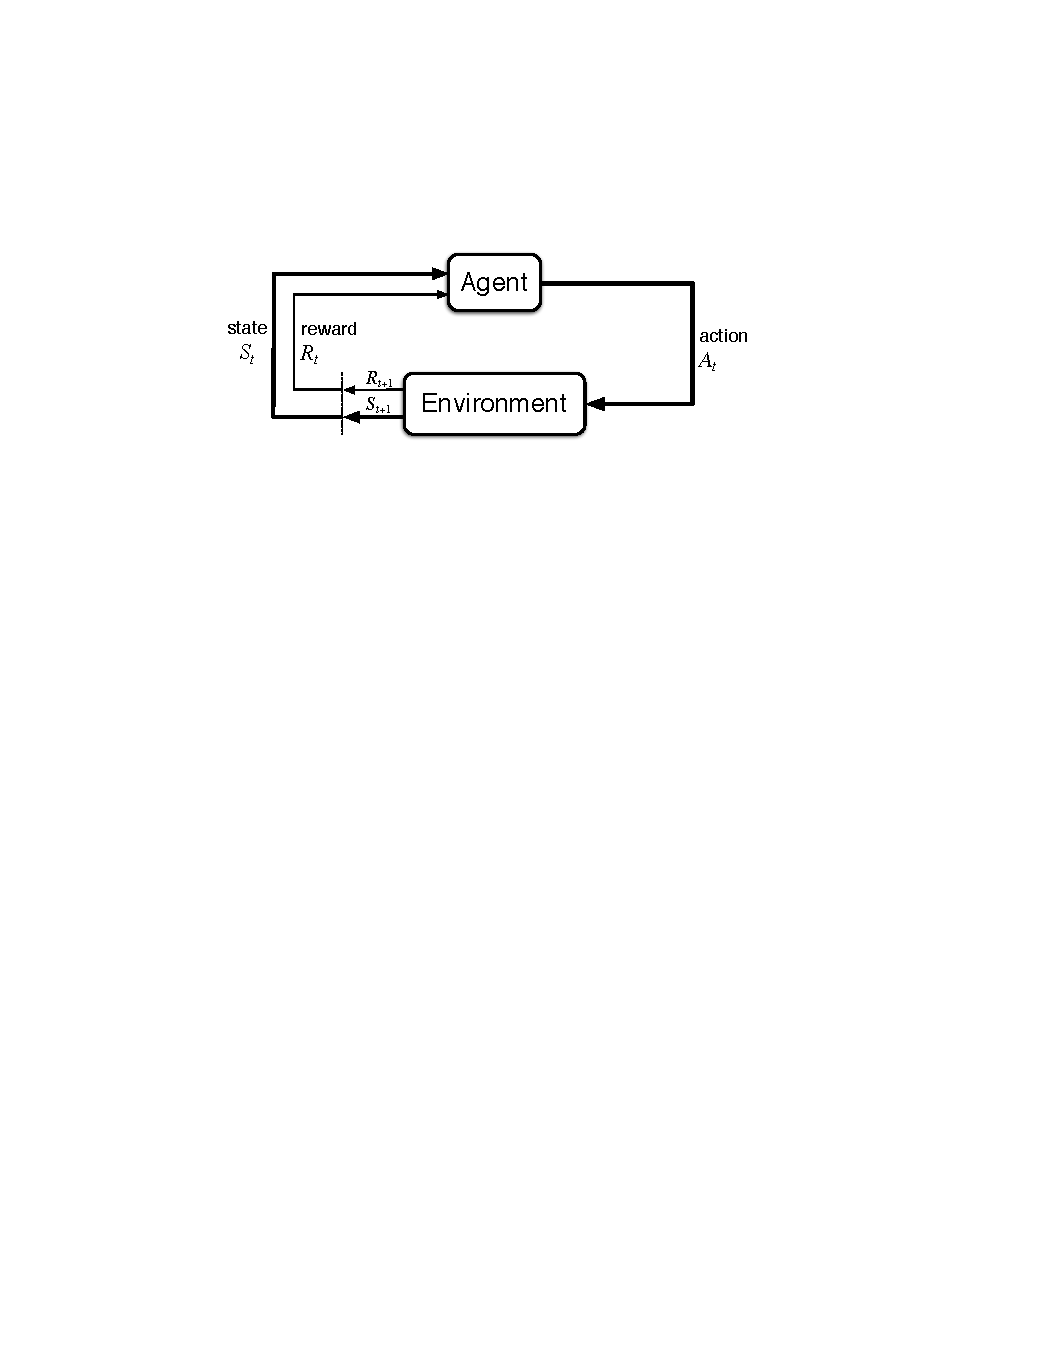
\includegraphics[width=0.8\textwidth]{rl-flowchart} 
    \caption[The interaction between the agent and the
        environment in \gls{rl}.]
    {The interaction between the agent and the
        environment in \gls{rl}%
        ~\cite[Fig.~3.1]{Sut20}.} 
    \label{fig:rl-flowchart} 
\end{figure}

According to the literature review, 
the combination of Gazebo, \gls{ros}
and \textsc{px4} are the most widely used software stack 
for the \gls{sitl} development,
which is a process that involves running the compiled code
used for the physical device in visual simulation environment.
The reason for their popularity is most likely 
due to their open-source nature. 
In contrast, Sphinx and Olympe, which are used in this project, 
are closed-source.
Although open-source software 
allows for full control and the flexibility to tinker
since the source code is freely available,
it is less stable and time-consuming to debug
when there is an error in the source code.
Another conclusion from the literature is that 
the transfer from simulation to the real world,
which this project also aims to accomplish,
is lacking in the studies reviewed.
As a result, it is not possible to comment on 
how the simulation findings effectively translate
into the physical environment.
% }}}}

% {{{{ background idea #3 
The third and final concept of the project 
is hardware realization for target visitation by a \gls{uav}.
This concept refers to building the physical world
that the simulation imitates in order to 
verify and validate the performance of the simulation.
The hardware part is essential in the implementation 
in the real world, where the simulation 
sometimes strays from the reality.
There is also a lack of hardware implementations in 
the field of research regarding drones with \gls{drl}, 
and most of the research papers focus on simulations.
According to the literature review, the \gls{cnn} 
models were used in the majority of the papers for object detection. 
Moreover, the controller boards and custom drone kits 
were used instead of commercial drones.
Those kits give researchers and users more flexibility 
since the drone is customizable 
in hardware and software. 
However, in design of the present research, 
a commercial drone will be used so that the research focuses 
on the \gls{drl}, but not on the actual drone building process. 
 
% }}}}

The relevant papers are analysed in a greater detail in
the succeeding \cref{sec:related-work} 
and summarized in \namecref{tab:lit-summary}~\ref{tab:lit-summary}.

\afterpage{
\begin{center}
    \begin{small}
        \begin{longtable}{ p{0.6cm} p{4cm} p{1.6cm} p{1.3cm} p{1.4cm} p{1.4cm} p{1.4cm} p{1.4cm} }
            \caption{Literature review summary
            \label{tab:lit-summary}} \\

            \toprule
            \textit{Ref} 
                & \textit{Main Objective} 
                    & \textit{Simulation} 
                        & \textit{Real-world} 
            & \textit{Single or Multi Drone} 
                & \textit{Technique} 
                    & \textit{Localizes Targets}  
                        & \textit{Mobile or Fixed Targets} \\
            \midrule
            \endfirsthead
            \caption[]{Literature review summary (continued)}\\
            \toprule
            \textit{Ref} 
                & \textit{Main Objective} 
                    & \textit{Simulation} 
                        & \textit{Real-world} 
            & \textit{Single or Multi Drone} 
                & \textit{Technique} 
                    & \textit{Localizes Targets}  
                        & \textit{Mobile or Fixed Targets} \\
            \midrule
            \endhead

            \cite{hua20}  
                & Minimize the time to scan targets and 
                propose a reactive real-time sliding 
                mode control algorithm to navigate a team 
                of \glspl{uav}. 
                    & Yes
                        & No 
            & Single and Multi 
                & Complex Math Calculations (\textsc{no ai}) 
                    & yes 
                        & mobile \\ \addlinespace

            \cite{pen21}  
                & To develop an online path planning 
                algorithm using \gls{drl}, minimize 
                energy consumption and maximize 
                offloaded data bits. 
                    & Yes 
                        & No 
            & Single 
                & Deep Reinforcement Learning 
                    & yes 
                        & mobile \\ \addlinespace

            \cite{hua21}
                & To navigate a team of unmanned 
                aerial vehicles (\glspl{uav}) to 
                monitor groups of ground pedestrians 
                and deliver a high-quality surveillance 
                    & Yes 
                        & Yes 
            & Multi 
                & Complex Math Calculations (\textsc{no ai}) 
                    &yes 
                        & mobile \\ \addlinespace

            \cite{Zho20}  
                & To adopt existing simulators and 
                propose a general framework to 
                incorporate \gls{dqn} algorithm with 
                the \gls{uav} simulation environment 
                    & Yes 
                        & \_ 
            &\_ 
                & \gls{drl} 
                     & \_ 
                         & \_ \\ \addlinespace

            \cite{Wal19}  
                 & To present the \gls{uav} indoor 
                 search problem two separate problems, 
                 a global planning problem and 
                 a local one, create a model to test 
                 the application of modern \gls{drl} 
                 approaches to the two problems. 
                    & Yes 
                        & No 
            & Single 
                & Deep Reinforcement Learning 
                    & \_ 
                        & \_ \\ \addlinespace

            \cite{Gar20} 
                & To use available software for 
                mission definition and execution in 
                \glspl{uav} based on PixHawk flight 
                controller and peripherals in 
                integrating and evaluating 
                a \gls{lidar} sensor 
                    & Yes 
                        & Yes 
            & Single 
                & Sensors 
                    & \_ 
                        & \_ \\ \addlinespace

            \cite{Zhao18} 
                & To build a deep learning model 
                that verifies the efficiency of 
                \gls{dl} for object detection 
                    & Yes 
                        & Yes 
            & Single 
                & Deep Learning and CNN 
                    & yes 
                        & mobile \\ \addlinespace

            \cite{Wang18} 
                & Create a powerful online drone 
                based moving target detection 
                for site inspection and 
                a violation detection tool 
                    & No 
                        & Yes 
            & Single 
                & Deep Learning and CNN 
                    & yes 
                        & mobile  \\

            \cite{Khan21}
                & To build integrate a deep 
                learning model in \glspl{uav} to spray 
                pesticides and monitor the crops.
                    & Yes 
                        & Yes 
            & Single 
                & Deep Learning and \gls{cnn} 
                    & yes 
                        & mobile \\ \addlinespace

            \bottomrule
        \end{longtable}
    \end{small}
\end{center}
}



\subsection{Related works}\label{sec:related-work}

In general, the relevant papers are divided into three main
categories. The first three sets of papers study
the different types of target visitation done by \uavs
and various techniques that were used to accomplish them. 
The next three papers concentrate on the use of simulation
to aid in achieving some tasks with a \uav.
Finally, the last three papers are concerned with designing
and testing a physical \uav system.
Reviewing these three areas of focus has helped us learn
from existing knowledge how to meet our objectives
and identified the gaps that our paper will attempt to 
address.

% {{{ Part 1
% #1
Related to the first category, authors in \cite{hua20} 
addressed a problem of autonomous navigation of \glspl{uav}. 
They proposed a reactive real-time sliding mode control algorithm 
that navigates a team of communicating \glspl{uav}.
The drones were equipped with ground-facing video cameras,
towards moving targets. 
Furthermore, they adopted the Voronoi partitioning \textsc{vp} technique 
to reduce the range of movement for each \gls{uav} and 
minimize the revisit time of each target as each drone was responsible 
for a sub-area.
They also ran extensive computer simulations using \textsc{matlab}. 
Their simulations of \textsc{matlab} were tried on one \gls{uav} and multiple \glspl{uav},
and they also considered the case of an uneven ground. 
Their main findings where that the use of the \textsc{vp} technique 
leads to more computation burden but can considerably reduce the target 
revisit time.

% #2

In~\cite{pen21}, the idea 
of taking advantage of \glspl{uav} in order to increase the network
coverage and execute computing tasks offloaded from multiple devices is studied. 
The constraints were to minimize the energy consumption of the \gls{uav} 
and maximize the amount of offloaded bits. 
Objects on the ground were not stationary and were following a Gauss-Markov 
movement pattern. Their approach was to apply \gls{drl} to develop an online path planning algorithm based on double deep Q-learning network (\textsc{ddqn}).
Simulations were also made to prove the viability of their idea and the 
effectiveness of the \gls{drl}-based path planning algorithm.

% #3
In a third paper, \cite{hua21} focused on navigating a team
of \glspl{uav} equipped with cameras to monitor groups of ground 
pedestrians or vehicles that were moving with a bounded speed with an unknown pattern. 
The surveillance is supposed to be from the shortest distances possible. 
They proposed an algorithm in which the \gls{uav} is able to determine 
its movement locally with some help from a central station.
Simulations were done to prove the algorithm's efficiency. However, the 
specific simulation software was not reviewed. 
% }}}

% {{{ Part 2

% {{{{ Zhou2020
% Topic sentence
The use of simulation makes rapid experiments in realistic settings 
and iterative \gls{uav} designs possible, 
both of which are important in \gls{ai} training. 
% Explanation
\citeauthor{Zho20} demonstrates this by % or \textcite{Zho20}
using a combination of the open-source 3D dynamic simulator Gazebo
and the autopilot system \textsc{px}4 
as shown in~\cref{fig:zho20}~\cite{Zho20}.
Through this, they avoided the time-consuming steps of 
carrying out physical experiments
and adjusting parameters according 
to the environmental settings~\cite{Zho20}.
Thanks to simulation, 
the authors were also able to propose a generic
framework to integrate the \gls{dqn} algorithm into 
the simulated \gls{uav} environment~\cite{Zho20}.
In our work, the same Gazebo physics engine
simulation software is used, and \gls{drl} is similarly trained
for the high-level control of the \gls{uav}. 
However, the authors used the \gls{ros}-\textsc{px}4 as the controller 
while in our work, the Olympe program is used.
The possible criticism against this paper could be the operating system,
which is Ubuntu 16.04 and 
the \gls{ros} version, Kinetic Kame that are old and are no longer supported 
even though the paper was written in 2020.
Nevertheless, the explanation and the flowchart illustrating the 
Q-learning in the context of drone control are instructive 
for our work to go forward.

\begin{figure}[b] 
    \centering
    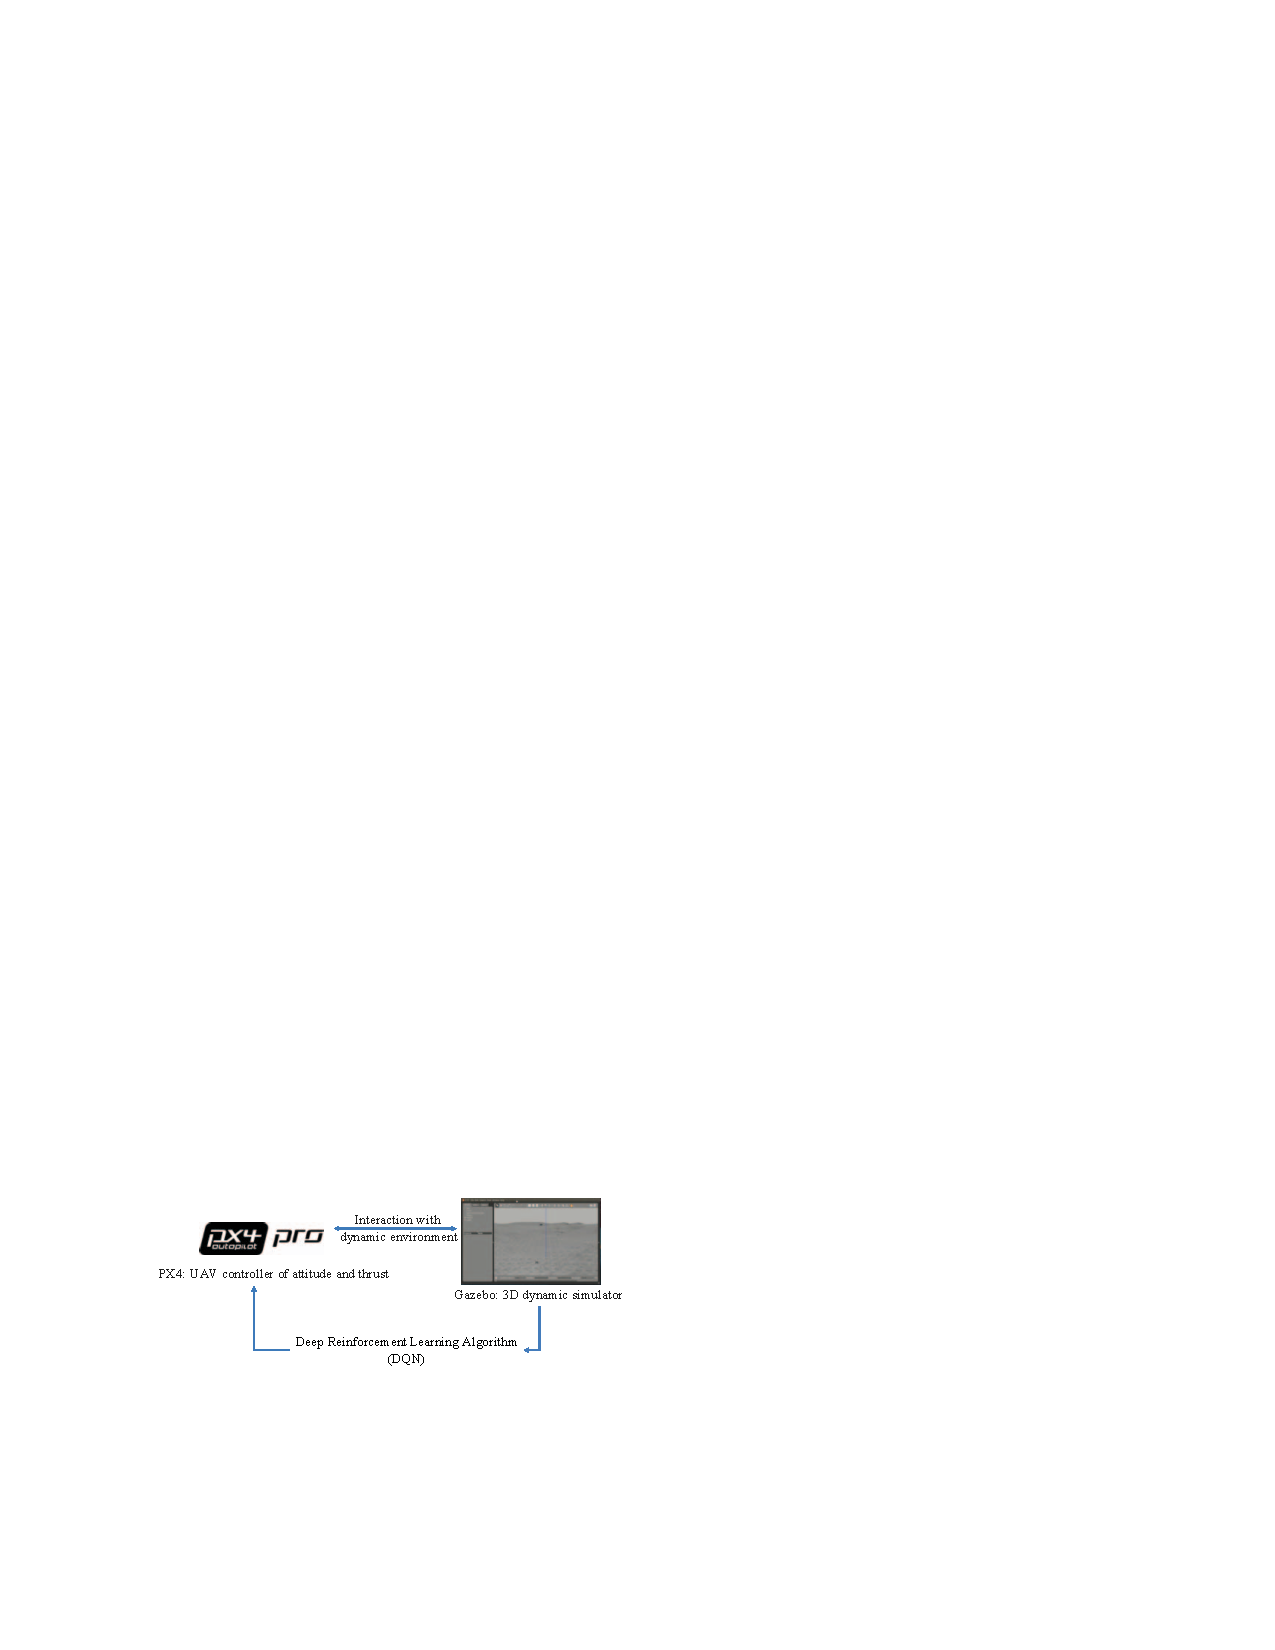
\includegraphics[width=0.9\textwidth]{zho20-flowchart} 
    \caption[The architecture of the framework proposed by
    \citeauthor{Zho20}.]
    {The architecture of the framework proposed by
    \citeauthor{Zho20}~\cite[Fig.~2]{Zho20}.} 
    \label{fig:zho20} 
\end{figure}
% }}}}

% {{{{ Walker2019
% Topic sentence
The time-saving benefit and the ease of experimentation 
afforded by the use of computer simulation are further emphasized 
when studying uncertain environments.
% Explanation
Dealing with an unknown environment for search and navigation applications,
\citeauthor{Wal19} used simulation to train a \gls{uav}
to solve a local planning problem
by framing the problem as 
a \gls{pomdp}
using continuous action spaces~\cite{Wal19}.
Similar to the previous paper, the \gls{ros}-\textsc{px4} stack 
and the Gazebo 
simulation software were used compared to Olympe and Sphinx 
in this project~\cite{Wal19}.
In addition, the present project and this paper planned with \gls{drl}, but the present work uses it for target visitation 
in an obstacle-free environment 
unlike the mentioned project which used it for searching and navigation
in both obstacle-free and non-obstacle-free environments.
However, the use of a \gls{uav} indoor by the authors as an application 
does not leverage the unique features of \glspl{uav}, 
but it is a good starting point 
and easier to implement in the real world 
when the outdoor flight is restricted.
A useful lesson that this paper provides for our project
is the use of the open \gls{ai} gym in creating the \gls{uav} environment,
resulting in clearer abstraction in the codebase
for the training process.
% }}}}

% {{{{ Garcia2020
% Topic sentence
Yet another \gls{uav} research-related applications 
that benefits from the use of computer simulation 
is the testing of new sensors on the \gls{uav}.
% Evidence 1
\citeauthor{Gar20} argued that the future of \glspl{uav}
relies on the use of advanced sensors and 
the ease of analyzing their functions
in real operational conditions~\cite{Gar20}.
% Response
To demonstrate such viability, they connected a \gls{lidar} sensor
to a Pixhawk flight controller and tested the improvement
that the new sensor provided
in the application of navigation and obstacle avoidance.
Importantly, prior to that, they used \textsc{qg}round\textsc{c}ontrol and the \textsc{px}4
platforms to analyze the addition of a \gls{lidar} sensor
on a simulated 3\textsc{dr} Iris \gls{uav} which is shown
in \cref{fig:gar20}.
Unlike our work, the authors' focus on using the simulation
was on sensor integration and not \gls{drl} 
which did not feature in the paper. 
The main criticism of this work is that 
the sensor is simulated without noise
when in the real world, the data captured
by the sensor is invariably noisy.
Although the objectives between the authors' and our work
are different, it is still very helpful to learn from
the extensive software stack and architecture guide 
presented by the authors.

\begin{figure}[tb] 
    \centering
    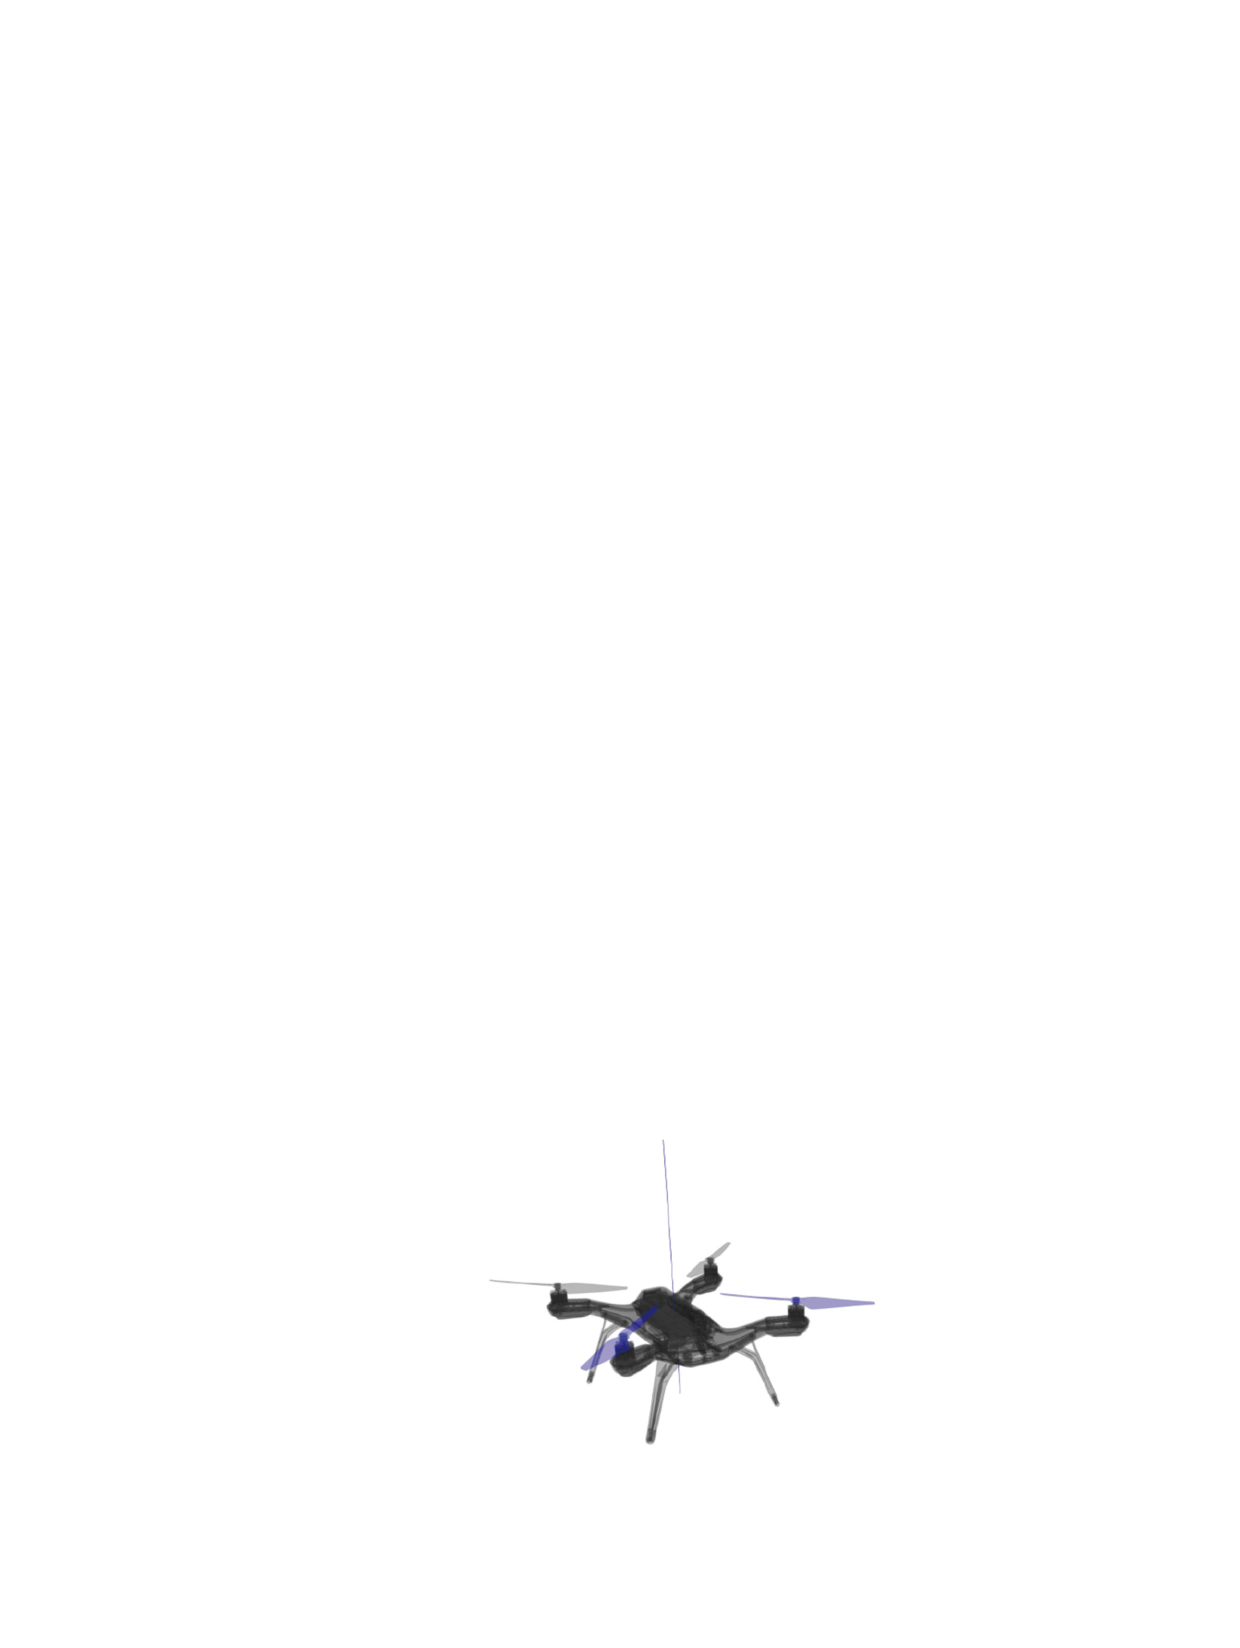
\includegraphics[width=0.5\textwidth]{gar20-iris} 
    \caption[The 3\textsc{dr} Iris model in the 
    Gazebo simulation used by \citeauthor{Gar20}.]
    {The 3\textsc{dr} Iris model in the 
    Gazebo simulation used by 
    \citeauthor{Gar20}~\cite[Fig.~4]{Gar20}.} 
    \label{fig:gar20} 
\end{figure}
% }}}}

% }}}

% {{{ Part 3

% Related work
% {{{{ Khan2021
% Topic sentence
With regards to the third category of papers,
\citeauthor{Khan21} used the drone in the agriculture field to spray 
pesticides and monitor crops. Unlike our work, the drone was limited to specific
boundaries and fixed targets such as crops.
They used a Raspberry Pi microcomputer board attached to the drone, which handles two different operations. Firstly, it controls the drone using an open-source
software called Arducopter autopilot which  handles the trip of the drone and the autonomous 
flights option. The second operation is to deal with the Intel neural computer stick 2, which will deploys the \gls{cnn} model and deals with the computation part~\cite{Khan21}.
Although this work is close to ours in terms of hardware, However there are some differences, 
one of which is using a custom drone which is not considered in our project since we are limited in time.
Since the \anafi drone will be used, the Olympe program will take control of the drone, which will
be installed on the Raspberry Pi. Finally, using \gls{cnn} only is not enough without \gls{drl} 
which makes the drone more intelligent and accurate.
% }}}}

% {{{{ Wang2018
% Topic sentence
In addition, commercial drones with an onboard computer use an \textsc{sdk} with image processing techniques.
% Explanation
The hardware architecture in \citeauthor{Wang18} includes a \textsc{dji} 
commercial drone and an onboard computer called manifold, which is from the same manufacturer.
Camera, onboard sensors like,\gls{gps} and inertial sensor are also included. Finally, an external battery for the manifold computer and Wi-Fi adapter that is used for the connection between the drone and the onboard computer will be needed. This hardware architecture is inspirational, and our design is somehow close to it with minor changes in the onboard computer and 
without the existence of the sensors. Besides, image and video processing techniques were used, such as 
segmentation to keep detecting moving targets as presented in~\cite{Wang18}.
For the navigation part, they used predetermined waypoints related to a historical path cost. 
However, in our work, probability and mobility patterns will be used to guess the target's location.
% }}}}

% {{{{ Zhao2018
% Topic sentence
The use of embedded system attached to the \gls{uav} which implements mobility pattern recognition will be used to decrease response time and save transmission bandwidth. 
% Explanation 
\citeauthor{Zhao18} used a quadrotor \gls{uav} supported with \gls{gps} module and a 
Pixhawk flight controller. The power sources in the architecture were two lithium batteries, 
one for the drone and one for the embedded system. The system uses \textsc{nvidia} Jetson development
kits which give enough computing power for the processing and communication between the flight 
controller and the system. The Jetson board is connected to the flight controller using serial 
communication while connected to the ground controller using Wi-Fi. Communication tools and protocols used in work by \citeauthor{Zhao18} will help us to determine the best way to communicate between the development board and the drone without any delay or interference~\cite{Zhao18}. 
% }}}}

% }}}

\end{document}
	
